\subsection{Binary Search}
Binary search algorithm is used to find elements in sorted structures. The benchmark program looks for integers in a sorted array of integers. The basic idea of the algorithm is to compare the integer to find with the middle element of the array. If the integer is larger than the middle element then the lower half of the array can be discarded and search can be focused on the top half. It the integer is smaller then search can be focused on the lower half. This process is repeated until the element matches the middle or search narrows down to an empty array. If search narrows down to an empty array then element is declared not found. The worst case for this algorithm happens when the element is not found and all narrowing steps must be completed in order to reach the conclusion that the item is not in the array. For example, if an array has 8192 $(2^{13})$ elements then 13 narrowing steps are required for the search in the worst case.

The idea of approximation in the case is to start search from a small subset array instead of the whole array. If the approximate position where the element may be found is known then we can look in the neighborhood of that location for the element. If the element is not found we can declare that the element is not in the array. For example, if we look in a neighborhood of size 64 $(2^{8})$ then only 8 narrowing steps are required to find an answer. The reduction in narrowing steps results in a speed up.

For this project the estimate of position is obtained through linear interpolation. This assumption here is that the items are drawn from a uniform distribution. In an array with 8192 $(2^{13})$ elements with a maximum (last element) of 32000 and least element (first element) of 0, the expected position of 12000 is given by (12000 * 8192) / (32000 - 0) = 3072. This defines a size 64 neighborhood ranging from positions 3040 to 3104. This approximation can never find an element which is not in the array therefore there are no false positives. But it is possible to miss elements that are in the array i.e. false negatives are possible.

The size of the neighborhood is the approximation knob in this case. We vary the size of the neighborhood from 1 to 2048 in arrays of size 8192. 10 arrays of size 8192 are drawn from a uniform distribution. For a sample measurement, one of the 10 arrays is selected first, then an element is selected at random from the array. This element is looked up using the approximate binary search. In this experiment 10000 samples are used for each knob value. The accuracy is defined as percentage of the elements found successfully in 10000 queries. Table \ref{bsearchT} present the accuracy numbers and the WCET estimate using PLATIN. WCET is represented as a percentage of the exact calculation time. In this case the timing estimate is for the complete application and includes initialization time as well.

\begin{table}[]
  \centering
  \caption{Binary Search Results}
  \label{bsearchT}
  \begin{tabular}{|l|l|l|}
    \hline
    \textbf{Neighborhood Size} & \textbf{Accuracy}     & \textbf{WCET}           \\ \hline
1 &  1.79
&65.81   \\ \hline
2 &  4.86
&69.33   \\ \hline
4 &  8.09
&72.55   \\ \hline
8 &  13.29
&75.88   \\ \hline
16 &  23.01
&79.20   \\ \hline
32 &  41.15
&82.53   \\ \hline
64 &  66.38
&85.85   \\ \hline
128 &  96.77
&89.17   \\ \hline
256 &  100.00
&92.50   \\ \hline
512 &  100.00
&95.82   \\ \hline
1024 &  100.00
&99.15   \\ \hline
2048 &  100.00
&102.47   \\ \hline
  \end{tabular}
\end{table}


The results show the following with respect to our questions:

\begin{enumerate}
\item We observe that a neighborhood size of 256 is enough to give us 100\% accuracy.
\item WCET increases linearly with log(Neighborhood Size). This relation is shown clearly in figure \ref{binarysearch2}.
  \item Accuracy reaches 100\% corresponding to a window size of 256. This corresponds to 92.5\% WCET.
\end{enumerate}

\begin{figure}
  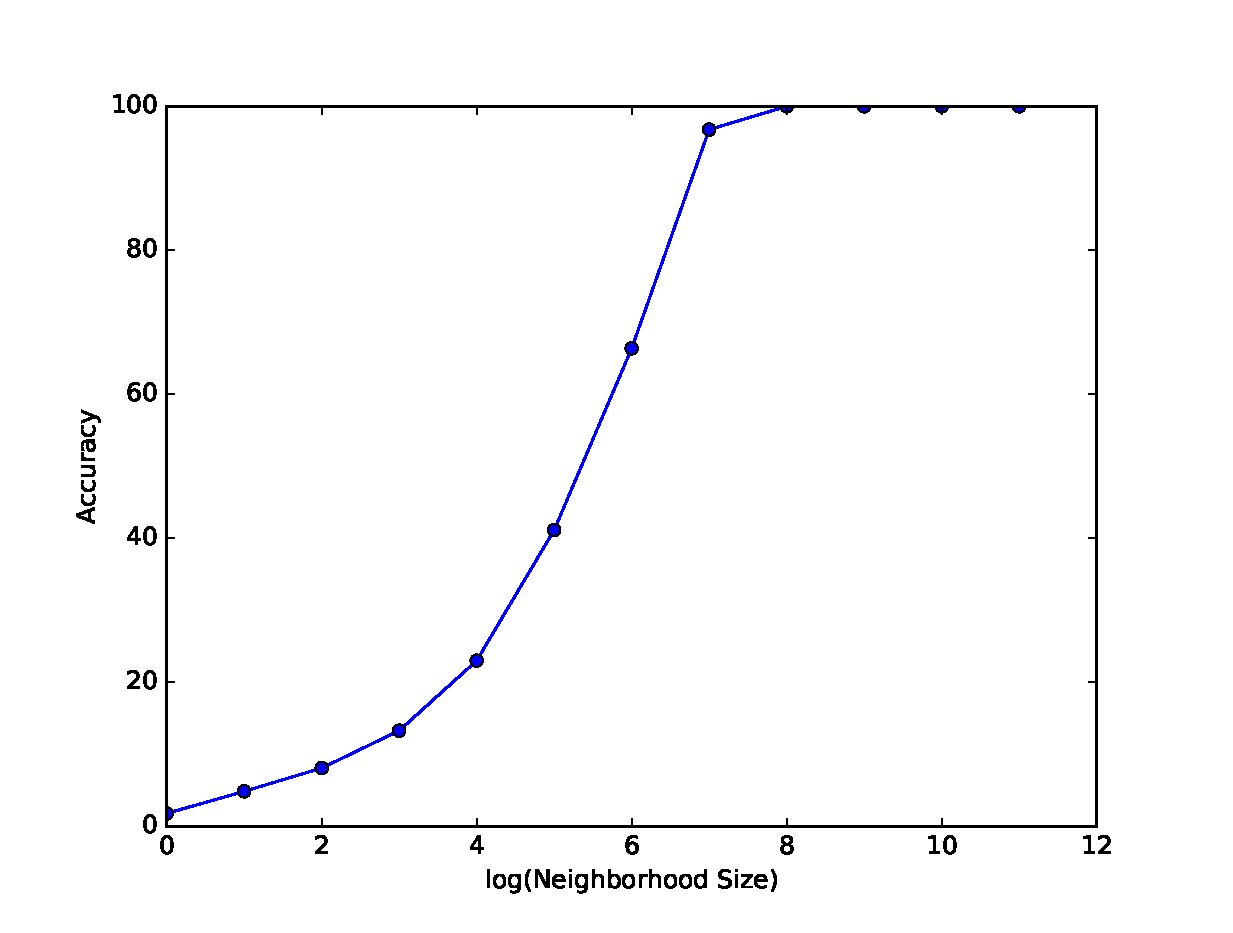
\includegraphics[width=0.95\linewidth]{Results/binarysearch1.eps}
  \caption{WCET vs log(Neighborhood Size)}
  \label{binarysearch2}
\end{figure}

The results show a potential saving of 8.5\% time. This saving can be used to save energy by running at 8.5\% slower rate or it can be used to make faster systems. This should only be used when the system designer is sure that input is uniformly distributed.

%% \begin{figure}
%%   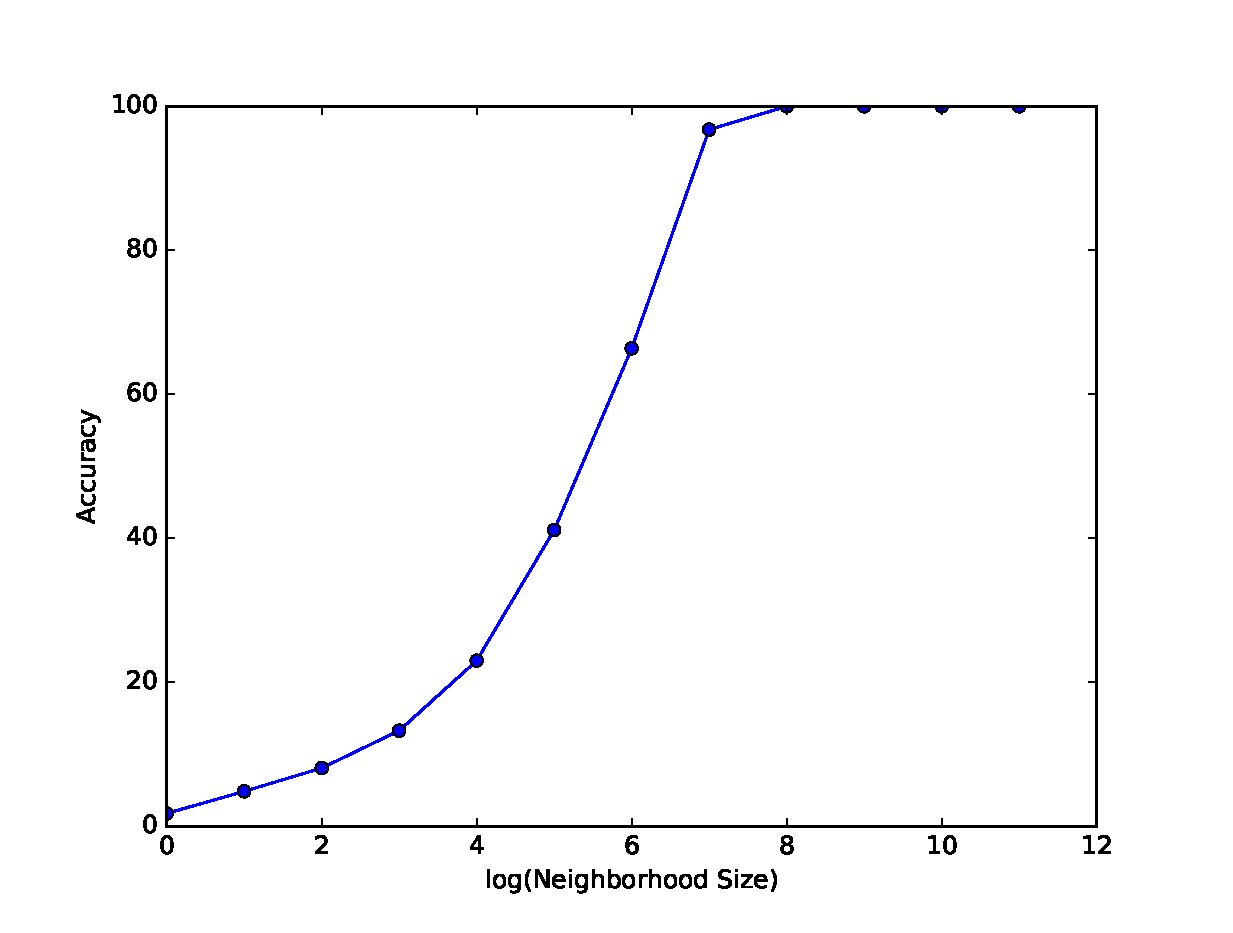
\includegraphics[width=0.95\linewidth]{Results/binarysearch1.eps}
%%   \caption{Accuracy vs log(Neighborhood Size)}
%%   \label{binarysearch1}
%% \end{figure}

%% \begin{figure}
%%   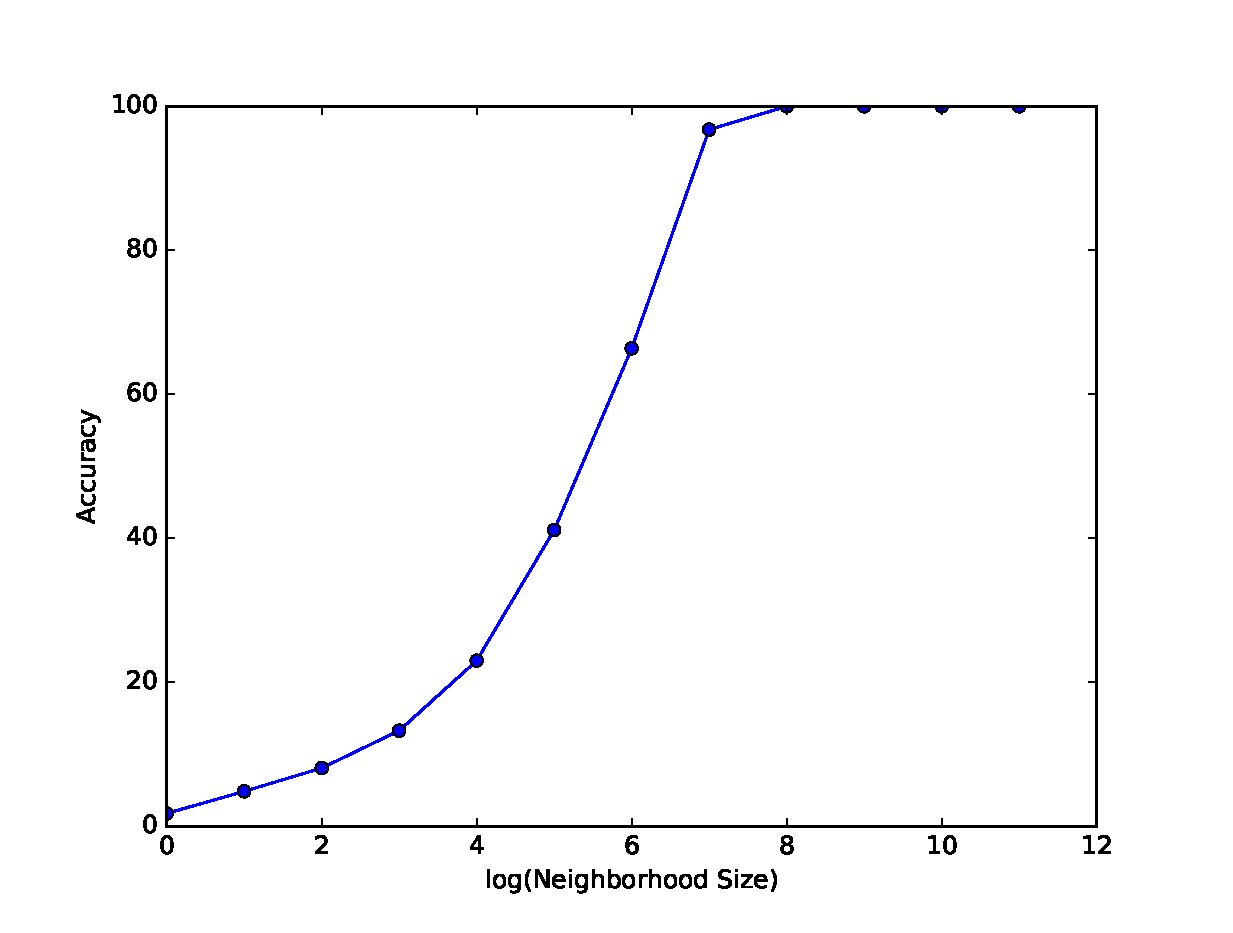
\includegraphics[width=0.95\linewidth]{Results/binarysearch1.eps}
%%   \caption{WCET vs Accuracy}
%%   \label{binarysearch3}
%% \end{figure}



